\documentclass[12pt, a4paper]{article}

% Packages and Formatting
\usepackage{../sub/mystyle_general}
\usepackage{../sub/mystyle_article}


\title{Intra-daily 51 Financial Factors Database}
\author{Guilherme Masuko \\
Advisor: Marcelo C. Medeiros}
\date{April 2023}
%\affil{}


\begin{document}

% Title Page
\begin{titlepage}
\clearpage
\maketitle
\thispagestyle{empty}
\begin{abstract}
	This paper had as main goal to report how we will create an intra daily basis of some of the key financial factors for the US market. In Section \ref{sec:data} we theoretically show how we form 51 factors. The final database will have 51 financial factors in addition to the returns of stocks listed on the US stock exchange NYSE. The main novelty in this database is the intra-daily frequency of these variables.
	
	During the scope of the article, we discussed the use of dimensionality reduction tools that will be needed in the context of model selection. We motivated this discussion by bringing the next steps that include verifying whether these factors help in the predictive power of high-frequency returns.
	
	
	%% PORTUGUESE VERSION
	
	%	Esse paper teve como principal objetivo reportar como criaremos uma base intra diária de alguns dos principais fatores financeiros para o mercado americano. Na Seção \ref{sec:data} mostramos teoricamente como formamos 51 fatores. A base de dados final contará com 51 fatores financeiros além dos retornos das ações listadas na bolsa americana NYSE. A principal novidade nesta base de dados é a frequência intra diária dessas variáveis.
	%	
	%	Durante o escopo do artigo, discutimos o uso de ferramentas de redução de dimensionalidade que serão necessárias no contexto de seleção de modelo. Motivamos essa discussão trazendo os próximos passos que abrangem verificar se esses fatores ajudam no poder preditivo de retornos em alta frequência.
\end{abstract}
\end{titlepage}

% Introduction
	\section{Introduction} \label{sec:introduction}
	Within the predictive world of finance, financial economists try to find methods and models that can increasingly more accurately predict stock returns. There are several approaches and tools used in financial analysis. These techniques are used to analyze historical data and try to predict future stock market movements.

On the one hand, the literature walked for a long time trying to discover financial factors that could better explain the returns or that would increase the predictive power of models that already have significant factors when making forecasts of returns. The search for factors that explain the cross section of expected stock returns began a long time ago with its first model, the Capital Asset Pricing Model (CAPM) introduced by \citeonline{sharpe1964capital}, \citeonline{lintner1965security} and \citeonline{mossin1966equilibrium} independently , based on previous work by \citeonline{markowitz1952portfolio}, using only the market factor to explain stocks' excess returns.

The factors are formed through portfolios where there is a long and a short position. For example, to create the market factor, we use a long position on the market index of interest and short on the risk-free interest rate, that is, market return minus risk-free asset return.

Looking for more factors that increase the predictive power, the well-known Fama and French models emerged, respectively, the three-factor model in \citeonline{fama1992cross} and the five-factor model in \citeonline{fama2015five}.

The first model aggregates the factors related to size, SMB (Small minus Big), and value, HML (High minus Low), based respectively on the variables Market Capitalization and Book-to-Market ratio, keeping the market factor at your model. In the second model, the authors add two more factors related to profitability and investment. Defined analogously to the SMB and HML factors, the RMW (Robust minus Weak) factors are constructed from the difference between the returns of firms with robust (high) and weak (low) operating profitability and the CMA investment factor (Conservative minus Aggressive) constructed from the difference between the returns of companies that invest conservatively and companies that invest aggressively. Another factor related to momentum was also added to the Fama and French three-factor model by \citeonline{carhart1997persistence}. MOM (Monthly Momentum Factor) can be calculated by subtracting the equal weighted average of the lowest performing companies from the equal weighted average of the highest performing companies.

Now, with hundreds of financial factors released in the literature, the difficulty has become to tame this high dimensionality of factors.

On the other hand, there is still a great use of traditional methods, such as the use of autoregressive regression (AR). This is what is done in \citeonline{chinco2019sparse}, which is the article most closely linked to this work. In the article, the authors use the AR regression with three lags as a reference model in their main specifications, although they demonstrate that the number of lags does not matter with the problem addressed. The objective of the article is to show that the identification of predictors in finance using only the intuition of researchers would only work for long-term stable predictors.

In high-frequency finance with modern, large, fast, and complex financial markets, the process of selecting predictors requires efforts that go beyond researchers' intuition. And perhaps these long-term stable predictors are not suitable to explain intraday returns because they are not able to capture the effects that affect stock prices in the middle of a day. The paper's results show that statistical model selection tools can increase the predictive power of one-minute-ahead forecasts of benchmark models using out-of-sample fit and forecast-implied Sharpe ratios as measures of quality.

For model selection, the authors make use of LASSO (Least Absolute Shrinkage and Selection Operator) using three lags of all returns as candidate predictors. They ague the use of a dimension reduction tool because there are many predictor candidates. For example, in the month of January 2003 our sample contains $4500+$ stocks. By using three lags, we then have $3\cdot 4500+ = 13500+$ candidate predictors. It would take more than 34 trading days to do a simple one-minute OLS (Ordinary Least Squares) estimation (each day has 390 minutes/observations) and test the predictors.

With this high dimensionality of predictor candidates, a reduction tool is necessary and a researcher's intuition does not seem to be the right path for this scale. LASSO fits as a solution because it is able to identify unexpected and short-term predictors, suitable for an intraday financial predictive model. The initial hypothesis for using LASSO is to bet on sparsity, that is, if among the $13500+$ candidate predictors, only a few predictors, say $S$, actually help to predict the returns of an asset, then we can leverage to use LASSO, because it would be needed only a little more than $S$ observations to make predictions, this means that, since we don't have to worry about the weak estimators, LASSO can estimate the remaining parameters with far fewer observations. Thus, if there are only $S$ important predictors at each point in time, LASSO is adequate for estimating unexpected short-term parameters. We explain more about how LASSO works in Appendix \ref{apen:lasso}.

Although the paper obtains results that refer to gains in predictive power by combining LASSO with Benchmarks models, the selection of predictors is made based only on return lags. The factors literature is neglected and therefore, this work was motivated to verify what happens when we add to this predictive model a base that contains relevant financial factors.

This summer paper therefore aims to explain how the database will be created and report the next steps after that. The work is divided into two more sections. Section \ref{sec:data} addresses how the databases have been built so far and how theoretically the factors will be built. Section \ref{sec:conclusion} will motivate what the next steps will be after having the base ready.




%% PORTUGUESE VERSION

%Dentro do mundo preditivo de finanças, os economistas financeiros tentam encontrar métodos e modelos que possam cada vez mais, fazer uma previsão mais precisa dos retornos das ações. Existem diversas abordagens e ferramentas utilizadas na análise financeira. Essas técnicas são usadas para analisar dados históricos e tentar prever futuros movimentos do mercado de ações.
%
%Por um lado, a literatura caminhou por muito tempo tentando descobrir fatores financeiros que pudessem explicar melhor os retornos ou que aumentassem o poder preditivo de modelos que já possuem fatores significativos na hora de fazer previsões de retornos. A procura por fatores que expliquem o cross section de retornos esperados de ações começou há muito tempo com seu primeiro modelo, Capital Asset Pricing Model (CAPM) introduzido por \citeonline{sharpe1964capital}, \citeonline{lintner1965security} e \citeonline{mossin1966equilibrium} independentemente, com base no trabalho anterior de \citeonline{markowitz1952portfolio}, usando apenas o fator mercado para explicar o excesso de retorno das ações. 
%
%Os fatores são formados através de portfólios onde há uma posição comprada e uma vendida. Por exemplo, para se criar o fator de mercado, usamos uma posição comprada no índice de mercado de interesse e vendido na taxa de juros livre de risco, isso é, retorno de mercado menos retorno do ativo livre de risco. 
%
%Procurando por mais fatores que aumentem o poder preditivo, surgiram os conhecidos modelos de Fama e French, respectivamente, modelo de três fatores em \citeonline{fama1992cross} e modelo de cinco fatores em \citeonline{fama2015five}. 
%
%O primeiro modelo agrega os fatores relacionados ao tamanho, SMB (Small minus Big), e valor, HML (High minus Low), baseando-se respectivamente, nas variáveis Market Capitalization e razão Book-to-Market, mantendo o fator de mercado em seu modelo. No segundo modelo, os autores acrescentam ainda mais dois fatores relacionados à lucratividade e investimento. Definidos de forma análoga aos fatores SMB e HML, são os fatores RMW (Robust minus Weak) construído a partir da diferença entre os retornos das firmas com rentabilidade operacional robusta (alta) e fraca (baixa) e o fator de investimento CMA (Conservative minus Aggressive) construído a partir da diferença entre os retornos das empresas que investem de forma conservadora e das empresas que investem de forma agressiva. Outro fator relacionado ao momentum também foi adicionado ao modelo trifatorial de Fama e French por \citeonline{carhart1997persistence}. O MOM (Monthly Momentum Factor) pode ser calculado subtraindo-se a média ponderada igual das empresas com desempenho mais baixo a partir da média ponderada igual das empresas com desempenho mais alto. 
%
%Agora, com centenas de fatores financeiros lançados na literatura, a dificuldade passou a ser domar essa alta dimensionalidade de fatores.
%
%Por outro lado, ainda existe uma grande utilização de métodos tradicionais, como o uso de regressão autorregressiva (AR). Isso é o que é feito em \citeonline{chinco2019sparse}, que é o artigo mais intimamente ligado a este trabalho. No artigo, os autores utilizam a regressão AR com três defasagens como modelo de referência em suas principais especificações, embora demonstrem que o número de defasagens não importa com o problema abordado. O objetivo do artigo é mostrar que a identificação de preditores em finanças utilizando somente a intuição de pesquisadores só funcionaria para preditores estáveis de longa duração. 
%
%Em finanças de alta frequência com mercados financeiros modernos, grandes, rápidos e complexos, o processo de seleção de preditores exige esforços que vão além da intuição de pesquisadores. E talvez esses preditores estáveis de longa duração não sejam adequados para explicar retornos intra diários por não serem capaz de capturar os efeitos que afetam os preços de ações no meio de um dia. Os resultados do paper mostram que ferramentas estatísticas de seleção de modelo podem aumentar o poder preditivo de previsões de um minuto à frente de modelos benchmark usando out-of-sample fit e forecast-implied Sharpe ratios como medidas de qualidade. 
%
%Para a seleção de modelo, os autores fazem uso do LASSO (Least Absolute Shrinkage and Selection Operator) usando três defasagens de todos os retornos como preditores candidatos. Eles defendem o uso de uma ferramenta de redução de dimensão por existirem muitos candidatos à preditores. Por exemplo, no mês de Janeiro de 2003 nossa amostra contém $4500+$ ações. Ao utilizar três defasagens, temos então $3\cdot 4500+ = 13500+$ candidatos a preditores. Seria necessário mais de 34 dias de negociações para fazer uma simples estimação OLS na frequência de um minuto (Ordinary Least Squares) (cada dia tem 390 minutos/observações) e testar os preditores. 
%
%Com essa alta dimensionalidade de candidatos a preditores, uma ferramenta de redução é necessária e a intuição de um pesquisador parece não ser o caminho adequado para essa escala. O LASSO se encaixa como solução por ser capaz de identificar preditores inesperados e de curta-duração, adequado para um modelo preditivo financeiro intra diário. A hipótese inicial para se usar o LASSO é apostar em sparsity, isso é, se dentre o $13500+$ candidatos a preditores, apenas alguns poucos preditores, digamos $S$, de fato ajudam a prever os retornos de um ativo, então podemos aproveitar para usar o LASSO, pois seria necessário apenas pouco mais de $S$ observações para fazer previsões, isso quer dizer que, como não precisamos nos preocupar com os estimadores fracos, o LASSO pode estimar os parâmetros remanescentes com muito menos observações. Assim, se existem apenas $S$ preditores importantes em cada ponto do tempo, o LASSO é adequado na estimação de parâmetros inesperados de curta-duração. Explicamos melhor como o LASSO funciona no Apêndice \ref{apen:lasso}.
%
%Embora o paper obtenha resultados que referem-se a ganhos no poder preditivo aliando o LASSO à modelos Benchmarks, a seleção de preditores é feita sobre apenas defasagens de retornos. A literatura de fatores é negligenciada e por isso, esse trabalho motivou-se em verificar o que acontece quando incrementamos à esse modelo preditivo uma base que contenha fatores financeiros relevantes.
%
%Esse artigo de verão tem como objetivo portanto, explicar como a base de dados será criada e reportar os próximos passos após isso. O trabalho está dividido em mais duas seções. A Seção \ref{sec:data} aborda como as bases de dados foram construídas até agora e como teoricamente, os fatores serão construídos. A Seção \ref{sec:conclusion} motivará quais serão os próximos passos após ter a base pronta.
% Data
	\section{Data} \label{sec:data}
	The first database of this work is TAQ Returns. The TAQ Returns database is a financial database that contains information on the returns of all stocks listed on the New York Stock Exchange (NYSE). We have around ten thousand assets entering and leaving the database from January 2003 to December 2020.

The TAQ Returns database provides return data at different frequencies, ranging from daily frequency to minute and second frequencies. For example, you can get return data for intervals such as 30, 15, 5, and 1 minute, as well as 30, 15, and 5 seconds. This allows for a more detailed and accurate analysis of stock performance over different time frames.

The second database was built using two different sets of data. The first contains data about PERMNO and TAQ\_TICKER. The second dataset also has the PERMNO column, which is the variable we connect the two datasets with, and several columns that give us the percentiles of companies on where they are located based on financial factors. Companies are grouped into ten percentiles. Thus, each firm receives values between 1 and 10.

With the TAQ Returns database and this last one together, we can construct some factors widely used in finance literature. We show below how these factors are constructed.


\begin{enumerate}
	\item \textbf{Size} ($size$)
	
	Based on \citeonline{fama1993common} we can built the first two factors, $size$ and $value$.
	
	\begin{align*}
		size &= \mathrm{ME}_{\text{Jun}} \\
	\end{align*}
	
	They construct six portfolios, $S/L, S/M, S/H, B/L, B/M, B/H$ from the intersections of two $\mathrm{ME}$ (Market Equity - price times shares) and three $\mathrm{BE}/\mathrm{ME}$ (Ratio of Book Equity to Market Equity) groups. The size breakpoint for year $t$ is the median NYSE market equity at the end of June of year $t$, breaking the first group $\mathrm{ME}$ into two, $S$ (Small) and $B$ (Big). The $SMB$ (Small minus Big) factor is, therefore, the average return on the three small portfolios minus the average return on the three big portfolios.
	
	\begin{align*}
		SMB &= \frac{1}{3}\left(S/L + S/M + S/H\right) - \frac{1}{3}\left(B/L + B/M + B/H\right)
	\end{align*}
	Rebalanced annually.


	
	\item \textbf{Value (annual)} ($value$)
	
	Follows \citeonline{fama1993common}. 
	
	\begin{align*}
		value &= \frac { \mathrm{BE} }{ \mathrm{ME} } \\
	\end{align*}

	 The $\mathrm{BE}/\mathrm{ME}$ group is broken into three book-to-market equity groups based on the breakpoints until the 30th $\mathrm{BE}/\mathrm{ME}$ percentile is $L$ (Low), from 30th until 70th percentile is $M$ (Middle) and finally the top 30th percentile $H$ (High). $\mathrm{BE}/\mathrm{ME}$ for June of year $t$ is the book equity for the last fiscal year end in $t-1$ divided by $\mathrm{ME}$ for December of $t-1$. The $HML$ (High minus Low) factor is the average return on the two high portfolios minus the average return on the two low portfolios. 
	
	\begin{align*}
		HML &= \frac{1}{2}\left(S/H + B/H\right) - \frac{1}{2}\left(S/L + B/L\right)
	\end{align*}
	Rebalanced annually.



	\item \textbf{Gross Profitability} ($prof$)
	
	Follows \citeonline{novy2013other}. 
	
	\begin{align*}
		prof &= \frac{ \mathrm{GP} }{ \mathrm{AT} } \\
	\end{align*}
	
	Profitability is measured by the ratio of a firm's gross profits (revenues minus cost of goods sold) to its assets. The gross profitability factor is constructed using the basic methodology employed in the construction of $HML$. The strategy are long (short) firms in the top (bottom) tertile by NYSE breaks on the profitability sorting variable. The returns of this portfolio are value-weighted and rebalanced annually at the end of June based on its performance over the first 11 months of the preceding year and gross profits-to-assets. The $PMU$ (Profitable minus Unprofitable) factor is 
	
	\begin{align*}
		PMU &= P - U
	\end{align*}
	where $GP$ is gross profits and $AT$ is total assets, $P$ and $U$ are, respectively, the value-weighted portfolio of the top 30th percentile and the bottom 30th percentile.
	
	
	
	\item \textbf{Value-Profitability} ($valprof$).
	
	Follows \citeonline{novy2013other}. 
	
	\begin{align*}
		valprof = \operatorname{rank}(value) + \operatorname{rank}(prof)
	\end{align*}
	Sum of ranks in univariate sorts on book-to-market and profitability. Annual book-to-market and profitability values are used for the entire year. Rebalanced annually.
	
	The strategy that the author consider is construct within the 500 largest non-financial stocks for which gross profits-to-assets and book-to-market are both available. Each year these stocks are ranked on both their gross profits-to-assets and book-to-market ratios, from 1 (lowest) to 500 (highest). At the end of each June the strategy buys one dollar of each of the 150 stocks with the highest ($H$) combined profitability and value ranks, and it shorts one dollar of each of the 150 stocks with the lowest ($L$) combined ranks.
		
	\begin{align*}
		HML = H - L
	\end{align*}
	
	
	
	\item \textbf{Piotroski's F-score} ($F$-$score$)
	
	Follows \citeonline{piotroski2000value}. 
	
	\begin{align*}
		F\text{-}score = & 1_{\text{IB}>0} + 1_{\Delta \text{ROA}>0} + 1_{\text{CFO}>0} + 1_{\text{CFO}>\text{IB}} + 1_{\Delta \text{DTA}<0 | \text{DLTT}=0 | \text{DLTT}_{-12}=0} \\
		& + 1_{\Delta \text{ATL}>0} + 1_{\text{EqIss} \leq 0} + 1_{\Delta \text{GM}>0} + 1_{\Delta \text{ATO}>0}
	\end{align*}
	where $\mathrm{IB}$ is income before extraordinary items, $\mathrm{ROA}$ is income before extraordinary items scaled by lagged total assets, $\mathrm{CFO}$ is cash flow from operations, $\mathrm{DTA}$ is total long-term debt scaled by total assets, $\mathrm{DLTT}$ is total long-term debt, $\mathrm{ATL}$ is total current assets scaled by total current liabilities, $\mathrm{EqIss}$ is the difference between sales of common stock and purchases of common stock recorded on the cash flow statement, $\mathrm{GM}$ equals one minus the ratio of cost of goods sold and total revenues, and $\mathrm{ATO}$ equals total revenues, scaled by total assets. Rebalanced annualy.
	
	
	
	\item \textbf{Debit Issuance} ($debtiss$)
	
	Follows \citeonline{spiess1999long}. 
	
	\begin{align*}
		debtiss = 1_{\text{DLTISS} \leq 0}
	\end{align*}
	Binary variable equal to one if long-term debt issuance indicated in statement of cash flow. Updated annually.
	
	
	
	\item \textbf{Share Repurchases} ($repurch$)
	
	Follows \citeonline{ikenberry1995market}. 
	
	\begin{align*}
		repurch = 1_{\text{PRSTKC>0}}
	\end{align*}
	Binary variable equal to one if repurchase of common or preferred shares indicated in statement of cash flow. Updated annually.
	
	
	
	\item \textbf{Share Issuance (annual)} ($nissa$)
	
	Follows \citeonline{pontiff2008share}. 
	
	\begin{align*}
		nissa = \frac{ \mathrm{shrout}_{\mathrm{Jun}} }{ \mathrm{shrout}_{\mathrm{Jun-12}} }
	\end{align*}	
	where shrout is the number of shares outstanding. Change in real number of shares outstanding from past June to June of the previous year. Excludes changes in shares due to stock dividends and splits, and companies with no changes in shrout.
	
	
	
	\item \textbf{Accruals} ($accruals$) 
	
	Follows \citeonline{sloan1996stock}. 
	
	\begin{align*}
		accruals =\frac{\Delta \mathrm{ACT}-\Delta \mathrm{CIIE}-\Delta \mathrm{LCT}+\Delta \mathrm{DLC}+\Delta \mathrm{TXP}-\Delta \mathrm{DP}}{(\mathrm{AT}+\mathrm{AT}_{-12}) / 2}
	\end{align*}
	where $\Delta \mathrm{ACT}$ is the annual change in total current assets, $\Delta \mathrm{CHE}$ is the annual change in total cash and short-term investments, $\Delta \mathrm{LCT}$ is the annual change in current liabilities, $\Delta \mathrm{DLC}$ is the annual change in debt in current liabilities, $\Delta \mathrm{TXP}$ is the annual change in income taxes payable, $\Delta \mathrm{DP}$ is the annual change in depreciation and amortization, and $\left(\mathrm{AT}+\mathrm{AT}_{-12}\right) / 2$ is average total assets over the last two years. Rebalanced annually.
	
	
	
	\item \textbf{Asset Growth} ($growth$) 
	
	Follows \citeonline{cooper2008asset}. 
	
	\begin{align*}
		growth = \frac{ \mathrm{AT} }{ \mathrm{AT}_{-12} }
	\end{align*}	
	Rebalanced annually.
	
	\item \textbf{Asset Turnover} ($aturnover$) 
	
	Follows \citeonline{soliman2008use} and \citeonline{novy2013other}.
	
	\begin{align*}
		aturnover = \frac{ \mathrm{SALE} }{ \mathrm{AT} }
	\end{align*}	
	Sales to total assets. Rebalanced annually.
	
	Portfolios are constructed using a quintile sort, where Low ($L$) represents the lowest 20th percentile and High ($H$) represents the highest 20th percentile based on New York Stock Exchange (NYSE) break points, and are rebalanced each year at the end of June
	
	\begin{align*}
		HML = H - L
	\end{align*}
	
	
	
	\item \textbf{Gross Margins} ($gmargins$). 
	
	Follows \citeonline{novy2013other}.
	
	\begin{align*}
		gmargins = \frac{ \mathrm{GP} }{ \mathrm{SALE} }
	\end{align*}
	where $\mathrm{GP}$ is gross profits and $\mathrm{SALE}$ is total revenues. Rebalanced annually.
	
	Portfolios are constructed using a quintile sort, where Low ($L$) represents the lowest 20th percentile and High ($H$) represents the highest 20th percentile based on New York Stock Exchange (NYSE) break points, and are rebalanced each year at the end of June.
		
	\begin{align*}
		HML = H - L
	\end{align*}
	 
	 
	 
	\item \textbf{Dividend Yield} ($divp$) 
	
	Follows \citeonline{naranjo1998stock}. 
	
	\begin{align*}
		divp = \frac{ \mathrm{Div} }{ \mathrm{ME}_{\text{Dec}} }
	\end{align*}
	Dividend scaled by price. Both are measured in December of the year $t-1$ or $t-2$ (for returns in months prior to July). Rebalanced annually.
	
	
	
	\item \textbf{Earnings/Price} ($ep$)
	
	Follows \citeonline{basu1977investment}.
	
	\begin{align*}
		ep = \frac{ \mathrm{IB} }{ \mathrm{ME}_{\text{Dec}} }
	\end{align*}
	Net income scaled by market value of equity. Updated annually.
	
	
	
	\item \textbf{Cash Flow / Market Value of Equity} ($cfp$) 
	
	Follows \citeonline{lakonishok1994contrarian}. 
	
	\begin{align*}
		cfp = \frac{ \mathrm{IB} + \mathrm{DP} }{ \mathrm{ME}_{\text{Dec}} }
	\end{align*}
	Net income plus depreciation and amortization, all scaled by market value of equity measured at the same date. Updated annually.
	
	
	
	\item \textbf{Net Operating Assets} ($noa$)
	
	Follows \citeonline{hirshleifer2004investors}.
	
	\begin{align*}
		noa = \frac{ ( \mathrm{AT} - \mathrm{CHE}) - (\mathrm{AT} - \mathrm{DLC} - \mathrm{DLTT} - \mathrm{MIB} - \mathrm{PSTK} - \mathrm{CEQ} ) }{ \mathrm{AT}_{-12} }
	\end{align*}
	where $\mathrm{AT}$ is total assets, $\mathrm{CHE}$ is cash and short-term investments, $\mathrm{DLC}$ is debt in current liabilities, $\mathrm{DLTT}$ is long term debt, $\mathrm{MIB}$ is non-controlling interest, $\mathrm{PSTK}$ is preferred capital stock, and $\mathrm{CEQ}$ is common equity. Updated annually.
	
	
	
	\item \textbf{Investment} ($inv$).
	
	Follows \citeonline{chen2011alternative}.
	
	\begin{align*}
	inv = \frac{ \Delta \mathrm{PPEGT} + \Delta \mathrm{INVT} }{ \mathrm{AT}_{-12} }
	\end{align*}
	where $\Delta \mathrm{PPEGT}$ is the annual change in gross total property, plant, and equipment, $\Delta \mathrm{INVT}$ is the annual change in total inventories, and $\mathrm{AT}_{-12}$ is lagged total assets. Rebalanced annually, uses the full period.
	
	
	
	\item \textbf{Investment-to-Capital} ($invcap$). 
	
	Follows \citeonline{xing2008interpreting}. 
	
	\begin{align*}
		invap = \frac{ \mathrm{CAPX} }{ \mathrm{PPENT} }
	\end{align*}
	Investment to capital is the ratio of capital expenditure (Compustat item $\mathrm{CAPX}$) over property, plant, and equipment (Compustat item $\mathrm{PPENT}$).
	
	
	
	\item \textbf{Invetment Growth} ($growth$). 
	
	Follows \citeonline{xing2008interpreting}. 
	
	\begin{align*}
		growth = \frac{ \mathrm{CAPX} }{ \mathrm{CAPX}_{-12} }
	\end{align*}
	Investment growth is the percentage change in capital expenditure (Compustat item $(\mathrm{CAPX})$
	
	
	
	\item \textbf{Sales Growth} ($sgrouth$).
	
	Follows \citeonline{lakonishok1994contrarian}.
	
	\begin{align*}
		sgrowth = \frac{ \mathrm{SALE} }{ \mathrm{SALE}_{-12} }
	\end{align*}
	Sales growth is the percent change in net sales over turnover (Compustat item $\mathrm{SALE}$).
	
	
	
	\item \textbf{Leverage} ($lev$). 
	
	Follows \citeonline{bhandari1988debt}. 
	
	\begin{align*}
		lev = \frac{ \mathrm{AT} }{ \mathrm{ME}_{\text{Dec}} }
	\end{align*}
	Market leverage is the ratio of total assets (Compustat item $\mathrm{AT}$) over the market value of equity. Both are measured in December of the same year.
	
	
	
	\item \textbf{Return on Assets (annual)} ($roma$).
	
	Follows \citeonline{chen2011alternative}. 
	
	\begin{align*}
		roaa = \frac{ \mathrm{IB} }{ \mathrm{AT} }
	\end{align*}
	Net income scaled by total assets. Updated annually.
	
	
	
	\item \textbf{Return on Equity (annual)} ($roea$). 
	
	Follows \citeonline{haugen1996commonality}. 
	
	\begin{align*}
		roea = \frac{ \mathrm{IB} }{ \mathrm{BE} }
	\end{align*}
	Net income scaled by book value of equity. Updated annually.
	
	
	
	\item \textbf{Sales-to-Price} ($sp$).
	
	
	Follows \citeonline{barbee1996sales}. 
	
	\begin{align*}
		sp =\frac{ \mathrm{SALE} }{ \mathrm{ME}_{\text{Dec}} }
	\end{align*}
	Total revenues divided by stock price. Updated annually.
	
	
	
	\item \textbf{Growth in LTNOA} ($gltnoa$). 
	
	Follows \citeonline{fairfield2003accrued}. 
	
	\begin{align*}
		gltnoa = \mathrm{GRNOA} - \mathrm{ACC}
	\end{align*}
	Growth in Net Operating Assets minus Accruals, where 
	
	\begin{align*}
		\mathrm{GRNOA} &= \mathrm{NOA} - \mathrm{NOA}_{\text{-12}} \\
		\mathrm{NOA} &= \frac{ \mathrm{RECT} + \mathrm{INVT} + \mathrm{ACO} + \mathrm{PPENT} + \mathrm{INTAN} + \mathrm{AO} - \mathrm{AP} - \mathrm{LCO} - \mathrm{LO} }{ \mathrm{AT} } \\
		\mathrm{ACC} &= \frac{ \Delta\mathrm{RECT} + \Delta\mathrm{INVT} + \Delta\mathrm{ACO} - \Delta\mathrm{AP} - \Delta\mathrm{LCO} - \mathrm{DP} }{ \left( \Delta\mathrm{AT} / 2 \right) } \\
		\Delta\mathrm{RECT} &= \mathrm{RECT} - \mathrm{RECT}_{-12} \\
		\Delta\mathrm{INVT} &= \mathrm{INVT} - \mathrm{INVT}_{-12} \\
		\Delta\mathrm{ACO} &= \mathrm{ACO} - \mathrm{ACO}_{-12} \\
		\Delta\mathrm{AP} &= \mathrm{AP} - \mathrm{AP}_{-12} \\
		\Delta\mathrm{LCO} &= \mathrm{LCO} - \mathrm{LCO}_{-12} \\
		\Delta\mathrm{AT} &= \mathrm{AT} - \mathrm{AT}_{-12} \\
	\end{align*}
	where $\mathrm{RECH}$ = Receivables, $\mathrm{INVT}$ = Total Inventory, $\mathrm{ACO}$ = Current Assets, $\mathrm{AP}$ = Accounts Payable, $\mathrm{LCO}$ =  Current Liabilities (Other), $\mathrm{DP}$ = Depreciation and Amortization, $\mathrm{AT}$ = Assets, $\mathrm{PPENT}$ = Property, Plant, and Equipment (net), $\mathrm{INTAN}$ = Intangible Assets, $\mathrm{AO}$ = Assets (Other), $\mathrm{LO}$ = Liabilities (Other). Updated annually.
	
	

	\item \textbf{Momentum (6m)} ($mom$). 
	
	Follows \citeonline{jegadeesh1993returns}. 
	
	\begin{align*}
		mom = \sum_{l=2}^7 r_{t-l}
	\end{align*}
	Cumulated past performance in the previous 6 months by skipping the most recent month. Rebalanced monthly.
	
	
	
	\item \textbf{Industry Momentum} ($indmom$). 
	
	Follows \citeonline{moskowitz1999industries}. 
	
	\begin{align*}
		indmom = \operatorname{rank} \left( \sum_{l=1}^6 r_{t-l}^{\text{ind}} \right)
	\end{align*}
	In each month, the Fama and French 49 industries are ranked on their value-weighted past 6-months performance. Rebalanced monthly.
	
	
	
	\item \textbf{Value-Momentum} ($valmom$). 
	
	Follows \citeonline{novy2013other}. 
	
	\begin{align*}
		valmom =\operatorname{rank}(value) + \operatorname{rank}(mom)
	\end{align*}
	Sum of ranks in univariate sorts on book-to-market and momentum. Annual book-to-market values are used for the entire year. Rebalanced monthly.
	
	
	
	\item \textbf{Value-Momentum-Profitability} ($malmomprof$). 
	
	Follows \citeonline{novy2013other}. 
	
	\begin{align*}
		valmomprof =\operatorname{rank}(value) + \operatorname{rank}(prof) + \operatorname{rank}(mom)
	\end{align*}
	Sum of ranks in umivariate sorts on book-to-market, profitability, and momentum. Annual book-to-market and profitability values are used for the entire year. Rebalanced monthly.
	
	
	
	\item \textbf{Short Interest} ($shortint$). 
	
	Follows \citeonline{dechow1998relation}. 
	
	\begin{align*}
		shortint = \frac{ \text{Shares Shorted} }{ \text{Shares Outstanding} }
	\end{align*}	
	Updated monthly.
	
	
	
	\item \textbf{Momentum (1 year)} ($mom12$). 
	
	Follows \citeonline{jegadeesh1993returns}. 
	
	\begin{align*}
		mom12 = \sum_{l=2}^{12} r_{t-l}
	\end{align*}
	Cumulated past performance in the previous year by skipping the most recent month. Rebalanced monthly.
	
	
	
	\item \textbf{Momentum-Reversal} ($momrev$). 
	
	Follows \citeonline{jegadeesh1993returns}. 
	
	\begin{align*}
		momrev = \sum_{d=14}^{19} r_{t-l}
	\end{align*}
	Buy and hold returns from $t-19$ to $t-14$. Updated monthly.
	
	
	
	\item \textbf{Long-term Reversals} ($lrrev$). 
	
	Follows \citeonline{de1985does}. 
	
	\begin{align*}
		lrrev = \sum_{l=13}^{60} r_{t-l} 
	\end{align*}
	Cumulative returns from $t-60$ to $t-13$. Updated monthly.
	
	
	
	\item \textbf{Value (monthly)} ($valuem$). 
	
	Follows \citeonline{asness2013devil}. 
	
	\begin{align*}
		valuem = \frac{ \mathrm{BEQ}_{-3} }{ \mathrm{ME}_{-1} }
	\end{align*}
	Book-to-market ratio using the most up-to-date prices and book equity (appropriately lagged). Rebalanced monthly.
	
	
	
	\item \textbf{Share Issuance (monthly)} ($nissm$).
	
	Follows \citeonline{pontiff2008share}. 
	
	\begin{align*}
		nissm = \frac{ \mathrm{shrout}_{t-13} }{ \mathrm{shrout}_{t-1} }
	\end{align*}
	where $\mathrm{shrout}$ is the number of shares outstanding. Change in real number of shares outstanding from $t-13$ to $t-1$. Excludes changes in shares due to stock dividends and splits, and companies with no changes in $\mathrm{shrout}$.
	
	
	
	\item \textbf{PEAD (SUE)} ($sue$). 
	
	Follows \citeonline{foster1984earnings}. 
	
	\begin{align*}
		sue = \frac{ \mathrm{IBQ} - \mathrm{IBQ}_{-12} }{ \sigma_{\mathrm{IBQ}_{-24}:\mathrm{IBQ}_{-3} } }
	\end{align*}
	where $\mathrm{IBQ}$ is income before extraordinary items (updated quarterly), and $\sigma_{\mathrm{IBQ}_{-24}:\mathrm{IBQ}_{-3}}$ is the standard deviation of $\mathrm{IBQ}$ in the past two years skipping the most recent quarter. Earnings surprises are measured by Standardized Unexpected Earnings (SUE), which is the change in the most recently announced quarterly earnings per share from its value announced four quarters ago divided by the standard deviation of this change in quarterly earnings over the prior eight quarters. Rebalanced monthly.
	
	
	
	\item \textbf{Return on Book Equity} ($roe$). 
	
	Follows \citeonline{chen2011alternative}. 
	
	\begin{align*}
		roe = \frac{ \mathrm{IBQ} }{ \mathrm{BEQ}_{-3} }
	\end{align*}
	where $\mathrm{IBQ}$ is income before extraordinary items (updated quarterly), and $\mathrm{BEQ}$ is book value of equity. Rebalanced monthly.
	
	
	
	\item \textbf{Return on Market Equity} ($rome$). 
	
	Follows \citeonline{chen2011alternative}. 
	
	\begin{align*}
		rome = \frac{ \mathrm{IBQ} }{ \mathrm{ME}_{-4} }
	\end{align*}
	where $\mathrm{IBQ}$ is income before extraordinary items (updated quarterly), and $\mathrm{ME}$ is market value of equity. Rebalanced monthly.
	
	
	
	\item \textbf{Return on Assets} ($roa$). 
	
	Follows \citeonline{chen2011alternative}. 
	
	\begin{align*}
		roa = \frac{ \mathrm{IBQ} }{ \mathrm{ATC}_{-3} }
	\end{align*}
	Net income scaled by total assets. Updated quarterly.
	
	
	
	\item \textbf{Short-term Reversal} ($strev$). 
	
	Follows \citeonline{jegadeesh1990evidence}. 
	
	\begin{align*}
		strev = r_{t-1}
	\end{align*}	
	Return in the previous month. Updated monthly.
	
	
	
	\item \textbf{Idiosyncratic Volatility} ($ivol$). 
	
	Follows \citeonline{ang2006cross}. 
	
	\begin{align*}
		ivol = \operatorname{std} \left( R_{i,t} - \beta_i R_{M,t} - s_i SMB_t - h_i HML_t \right)
	\end{align*}
	The standard deviation of the residual from firm-level regression of daily stock returns on the daily innovations of the Fama and French three-factor model using the estimation window of three months. Lagged one month.
	


	\item \textbf{Beta Arbitrage} ($beta$). 
	
	Follows \citeonline{cooper2008asset}. 
	
	\begin{align*}
		beta = \beta_{t-60:t-1}
	\end{align*}
	Beta with respect to the CRSP equal-weighted return index. Estimated over the past 60 months (minimum 36 months) using daily data and lagged one month. Updated monthly.
	
	
		
	\item \textbf{Seasonality} ($season$). 
	
	Follows \citeonline{heston2008seasonality}. 
	
	\begin{align*}
		season = \sum_{l=1}^5 r_{t-l\operatorname{x}12}
	\end{align*}
	Average monthly return in the same calendar month over the last 5 years. As an example, the average return from prior Octobers is used to predict returns this October. The firm needs at least one year of data to be included in the sample. Updated monthly.
	
	
	
	\item \textbf{Industry Relative Reversals} ($indrrev$). 
	
	Follows \citeonline{da2014closer}. 
	
	\begin{align*}
		indrrev = r_{-1} - r^{ind}_{-1}
	\end{align*}
	where $r$ is the return on a stock and $r^ind$ is return on its industry. Difference between a stocks' prior month's return and the prior month's return of its industry (based on the Fama and French 49 industries). Updated monthly.
	
	
	
	\item \textbf{Industry Relative Reversals (Low Volatility)} ($indrrevlv$). 
	
	Follows \citeonline{da2014closer}. 
	
	\begin{align*}
		indrrevlv = r_{-1} - r^{ind}_{-1}
	\end{align*}
	if vol ¡ NYSE median, where $r$ is the return on a
	stock and rind is return on its industry. Difference between a stocks' prior month's return and the prior month's return of its industry (based on the Fama and French 49 industries). Only stocks with idiosyncratic volatility lower than the NYSE median for month are included in the sorts. Updated monthly.
	
	
	
	\item \textbf{Industry Momentum-Reversal} ($indmomrev$). 
	
	Follows \citeonline{moskowitz1999industries}. 
	
	\begin{align*}
		indmomrev = \operatorname{rank}(indmom) + \operatorname{rank}(indrrevlv)
	\end{align*}
	Sum of Fama and French 49 industries ranks on industry momentum and industry relative reversals (low vol). Rebalanced monthly.
	
	
	
	\item \textbf{Composite Issuance} ($ciss$). 
	
	Follows \citeonline{daniel2006market}. 
	
	\begin{align*}
		ciss = \log\left( \frac{ \mathrm{ME}_{t-13} }{ \mathrm{ME}_{t-60} } \right) - \sum^60_{l=13} r_{t-l}
	\end{align*}
	where $r$ is the log return on the stock and $\mathrm{ME}$ is total market equity. Updated monthly.
	
	
	
	\item \textbf{Price} ($price$). 
	
	Follows \citeonline{blume1973price}. 
	
	\begin{align*}
		price = \log\left( \frac{ \mathrm{ME} }{ \mathrm{shrout} } \right)
	\end{align*}
	where $\mathrm{ME}$ is market equity and $\mathrm{shrout}$ is the number of shares outstanding. Log of stock price. Updated monthly.
	
	
	
	\item \textbf{Firm Age} ($age$). 
	
	Follows \citeonline{barry1984differential}. 
	
	\begin{align*}
		age = \log(1 + \text{number of months since listing})
	\end{align*}
	The number of months that a firm has been listed in the CRSP database.
	
	
	
	\item \textbf{Share Volume} ($shvol$). 
	
	Follows \citeonline{datar1998liquidity}. 
	
	\begin{align*}
		shvol = \frac{1}{3} \sum^3_{i=1} \frac{ \mathrm{volume}_{t-i} }{ \mathrm{shrout}_t }
	\end{align*}
	Average number of shares traded over the previous three months scaled by shares out-standing. Updated monthly.
	
	
	
	\item \textbf{Cash flow duration} ($dur$). 
	
	Follows ?. 
	
	\begin{align*}
		dur = \frac{ \sum_t \mathrm{PV}_0 \left( t \times \mathrm{CF}_t \right) }{ P_0 }
	\end{align*}
	Present value of expected cashflows. Cashflows' components (from clean surplus identity, ROE and book equity growth) are forecasted using AR(1). Sums are discounted using a constant discount rate. Rebalanced monthly.
		
\end{enumerate}



%% PORTUGUESE VERSION

%A primeira base de dados deste trabalho é o TAQ Returns. O banco de dados TAQ Returns é um banco de dados financeiro que contém informações sobre os retornos de todas as ações listadas na Bolsa de Valores de Nova York (NYSE). Temos cerca de dez mil ativos entrando e saindo do banco de dados no período de janeiro de 2003 a dezembro de 2020.
%
%O banco de dados TAQ Returns fornece dados de retorno em diferentes frequências, variando de frequência diária a frequências por minuto e por segundo. Por exemplo, você pode obter dados de retorno para intervalos como 30, 15, 5 e 1 minuto, bem como 30, 15 e 5 segundos. Isso permite uma análise mais detalhada e precisa do desempenho das ações em diferentes intervalos de tempo.
%
%O segundo banco de dados foi montado usando dois conjuntos diferentes de dados. O primeiro contém dados sobre PERMNO e TAQ\_TICKER. O segundo conjunto de dados também possui a coluna PERMNO, que é a variável que conectamos os dois conjuntos de dados e várias colunas que nos fornecem o percentis de empresas sobre onde estão localizadas com base em fatores financeiros. As empresas estão agrupadas em dez percentis. Assim, cada firma recebe valores entre 1 e 10.
%
%Com o banco de dados TAQ Returns e este último juntos, podemos construir alguns fatores amplamente utilizados na literatura de finanças. Mostramos a seguir como esses fatores são construídos.
% Conclusion
	\section{Conclusion} \label{sec:conclusion}
	The main objective of this summer paper was to document the data manipulation process. We describe how we create portfolios related to some of the key financial factors documented in the literature. The final database contains daily intraday stock returns and financial factor portfolios.

In Section \ref{sec:introduction}, we briefly mentioned the goals after finalizing the database. The intention is to model through LASSO which predictor candidates among stock returns and portfolios of financial factors help to improve the predictive power of high-frequency asset pricing. Along the same line, we will be able to verify whether, unlike \citeonline{chinco2019sparse}, when including financial factors there is an increase in predictive power.

Next steps include adding more robust methods to evaluate which predictor candidates increase predictive power, such as the Double Selection LASSO featured in \citeonline{feng2020taming}. This procedure considers model selection errors by selecting predictors that not only help explain the cross-section of expected returns, but are also useful in mitigating the problem of omitted variable bias.

Furthermore, as LASSO is a tool whose predictor selection is based purely on a statistical rule, we would like to check whether there is economic meaning for the selected predictors through twitter data.



%% PORTUGUESE VERSION

%
%O objetivo principal deste paper de verão foi documentar o processo de manipulação dos dados. Descrevemos como criamos portfólios relacionados a alguns dos principais fatores financeiros documentados na literatura. A base de dados final contém retornos intra diários de ações e dos portfólios de fatores financeiros.
%
%Na Seção \ref{sec:introduction}, mencionamos brevemente os objetivos após a finalização da base de dados. A intenção é modelar através do LASSO quais candidatos a preditores dentre retornos de ações e dos portfólios de fatores financeiros ajudam a melhorar o poder preditivo de apreçamento de ativos em alta frequência. Nesta mesma linha, poderemos verificar se diferentemente de \citeonline{chinco2019sparse}, ao incluir fatores financeiros há um aumento no poder preditivo.
%
%Os próximos passos incluem a adição de métodos mais robustos para avaliar quais candidatos a preditores aumentam o poder preditivo, como o LASSO de Seleção Dupla apresentado em \citeonline{feng2020taming}. Esse procedimento considera erros de seleção de modelo ao selecionar preditores que não somente ajudam a explicar o cross-section de retornos esperados, mas também são úteis em mitigar o problema de viés de variável omitida. 
%
%Além disso, como o LASSO é uma ferramenta cujo a seleção de preditores se baseia puramente em uma regra estatística, gostaríamos de verificar se há significado econômico para os preditores selecionados através de dados do twitter.
% References
	\newpage
	\bibliographystyle{abntex2-alf}
	\bibliography{ref}
% Appendix
	\newpage
	\appendix
	\section{Appendix} \label{sec:appendix}
	\subsection{LASSO}\label{apen:lasso}

LASSO is a categorized procedure within the set of penalized regressions. Penalized Least Squares is a punishment procedure that adds to the OLS regression a component that penalizes weak coefficients. The Penalty Least Squares estimator is obtained through

\begin{align*}
	\widehat{\boldsymbol{\beta}}(\lambda)=\underset{\boldsymbol{\beta} \in \mathcal{B}}{\arg \min }\left[\sum_{i=1}^n\left(Y_i-\boldsymbol{\beta}^{\prime} \boldsymbol{X}_i\right)^2+\sum_{j=1}^p p_\lambda\left(\left|\beta_j\right| ; \boldsymbol{\alpha}, \text { data }\right)\right]
\end{align*}

where $p_\lambda\left(\left|\beta_j\right| ; \boldsymbol{\alpha}, \text{data}\right)$ is a non-negative penalty function indexed by the regularization parameter $\lambda$ and could rely on both the data and additional hyperparameters. For example,

\begin{itemize}
	\item Ridge
	
	$p_\lambda\left(\left|\beta_j\right| ; \boldsymbol{\alpha}\right.$, data $)=\lambda\left|\beta_j\right|^2$
	\item LASSO
	
	$p_\lambda\left(\left|\beta_j\right| ; \boldsymbol{\alpha}\right.$, data $)=\lambda\left|\beta_j\right|$
	\item LASSO and Ridge combined
	
	$p_\lambda\left(\left|\beta_j\right| ; \boldsymbol{\alpha}\right.$, data $)=\alpha \lambda\left|\beta_j\right|+(1-\alpha) \lambda\left|\beta_j\right|^2$
\end{itemize}

The regularization parameter $\lambda$ controls the number of parameters in the model. If $\lambda = \infty$, then no parameters enter the model, and if $\lambda = 0$, then the parameters are simply OLS estimators.



% FIGURES
\newpage
\subsection{Figures}


\begin{figure}[H]
	\caption{Number of stocks in each Database}
	\centering
	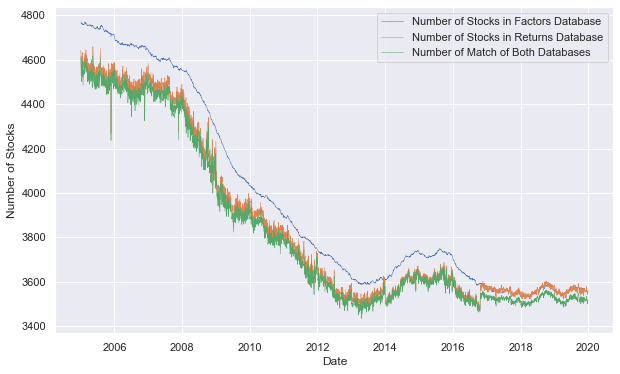
\includegraphics[scale=.73]{../../output/figures/match.png}
	\label{fig:match}
\end{figure}



\begin{figure}[H]
	\caption{Size Factor Returns Distribution}
	\centering
	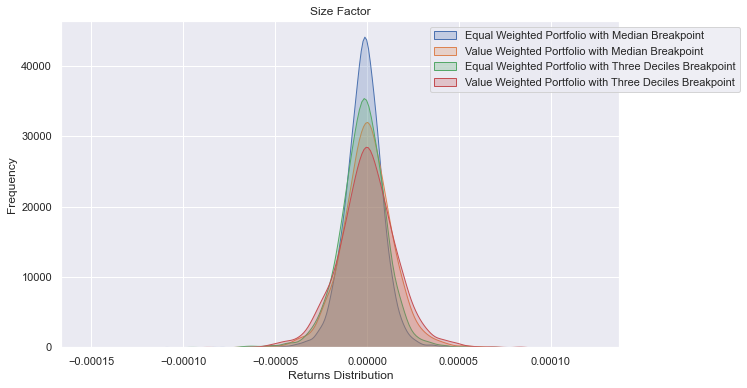
\includegraphics[scale=.63]{../../output/figures/size.png}
	\label{fig:size}
\end{figure}

\begin{figure}[H]
	\caption{Value Factor Returns Distribution}
	\centering
	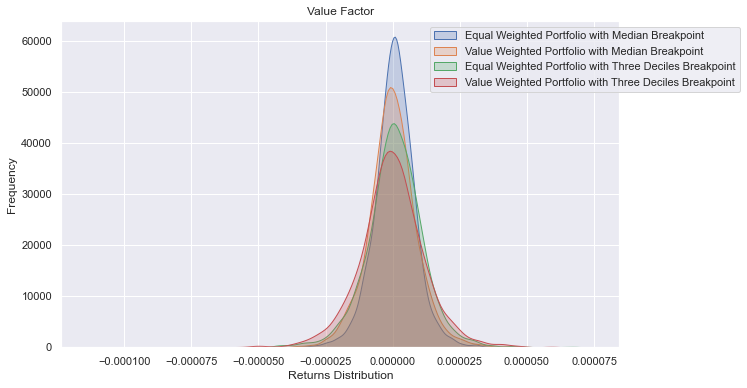
\includegraphics[scale=.63]{../../output/figures/value.png}
	\label{fig:value}
\end{figure}

\begin{figure}[H]
	\caption{Prof Factor Returns Distribution}
	\centering
	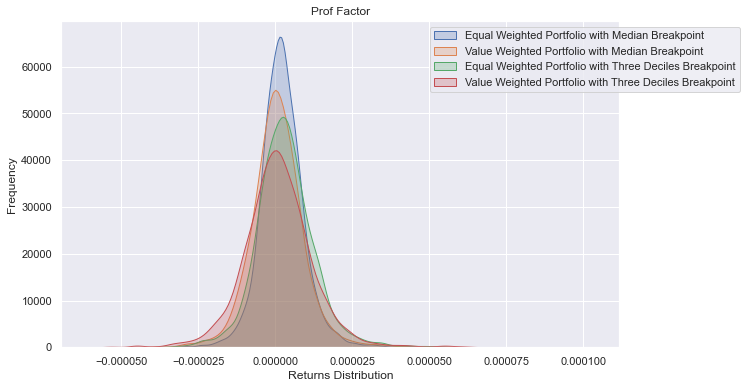
\includegraphics[scale=.63]{../../output/figures/prof.png}
	\label{fig:prof}
\end{figure}

\begin{figure}[H]
	\caption{Dur Factor Returns Distribution}
	\centering
	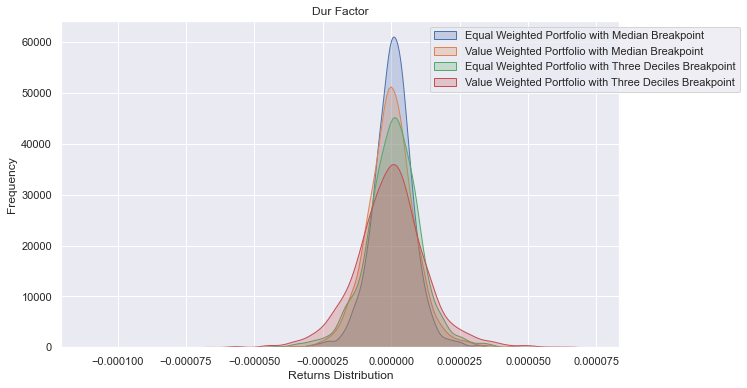
\includegraphics[scale=.63]{../../output/figures/dur.png}
	\label{fig:dur}
\end{figure}

\begin{figure}[H]
	\caption{Valprof Factor Returns Distribution}
	\centering
	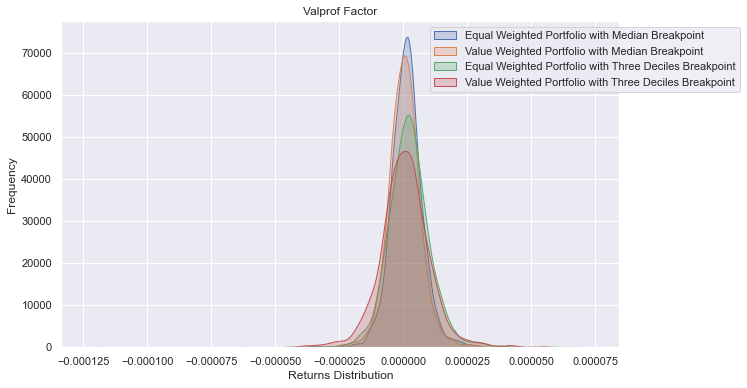
\includegraphics[scale=.63]{../../output/figures/valprof.png}
	\label{fig:valprof}
\end{figure}

\begin{figure}[H]
	\caption{Fscore Factor Returns Distribution}
	\centering
	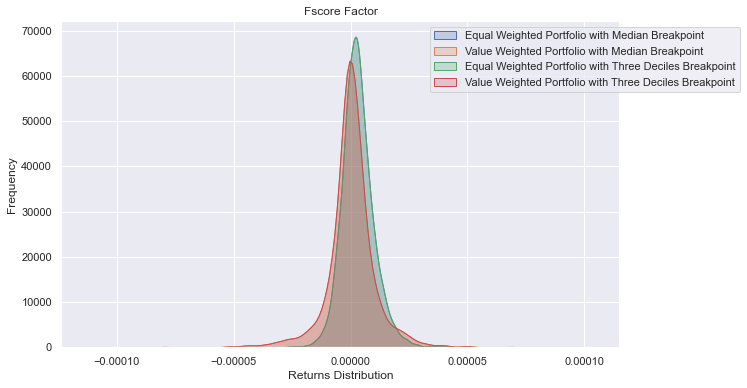
\includegraphics[scale=.63]{../../output/figures/fscore.png}
	\label{fig:fscore}
\end{figure}

\begin{figure}[H]
	\caption{Debtiss Factor Returns Distribution}
	\centering
	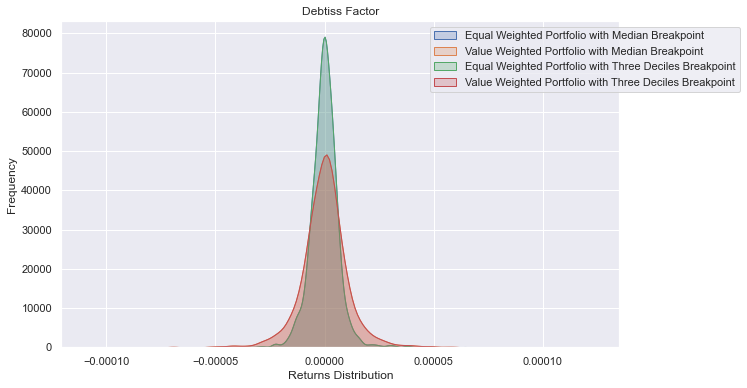
\includegraphics[scale=.63]{../../output/figures/debtiss.png}
	\label{fig:debtiss}
\end{figure}

\begin{figure}[H]
	\caption{Repurch Factor Returns Distribution}
	\centering
	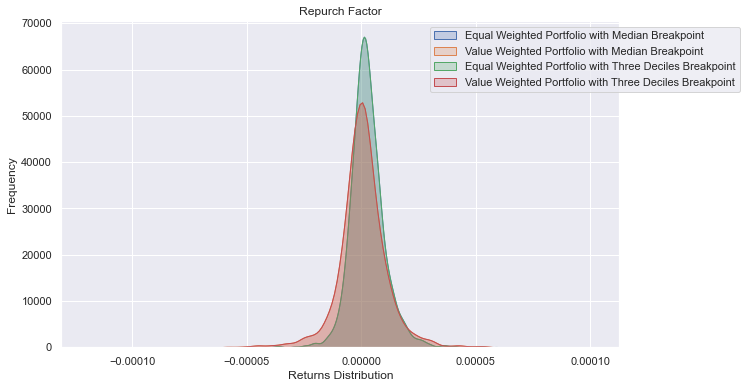
\includegraphics[scale=.63]{../../output/figures/repurch.png}
	\label{fig:repurch}
\end{figure}

\begin{figure}[H]
	\caption{Nissa Factor Returns Distribution}
	\centering
	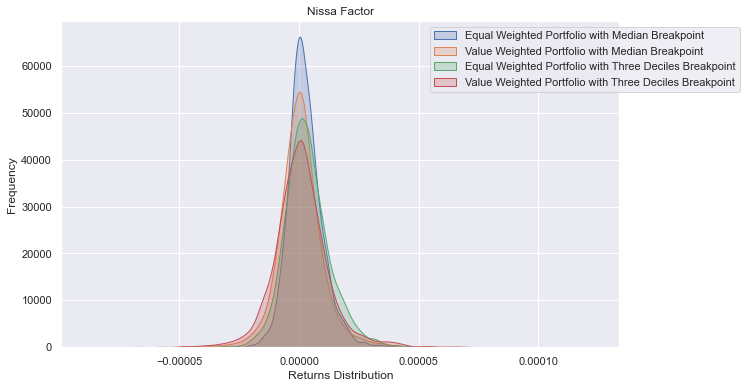
\includegraphics[scale=.63]{../../output/figures/nissa.png}
	\label{fig:nissa}
\end{figure}

\begin{figure}[H]
	\caption{Accruals Factor Returns Distribution}
	\centering
	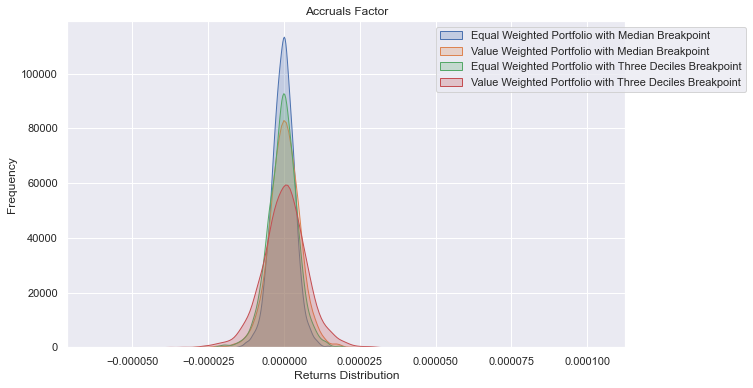
\includegraphics[scale=.63]{../../output/figures/accruals.png}
	\label{fig:accruals}
\end{figure}

\begin{figure}[H]
	\caption{Growth Factor Returns Distribution}
	\centering
	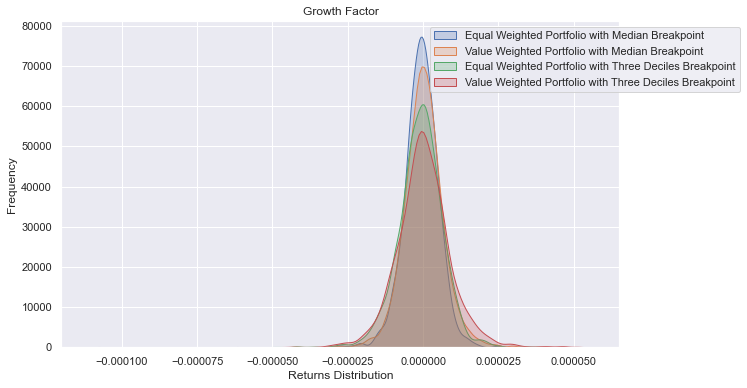
\includegraphics[scale=.63]{../../output/figures/growth.png}
	\label{fig:growth}
\end{figure}

\begin{figure}[H]
	\caption{Aturnover Factor Returns Distribution}
	\centering
	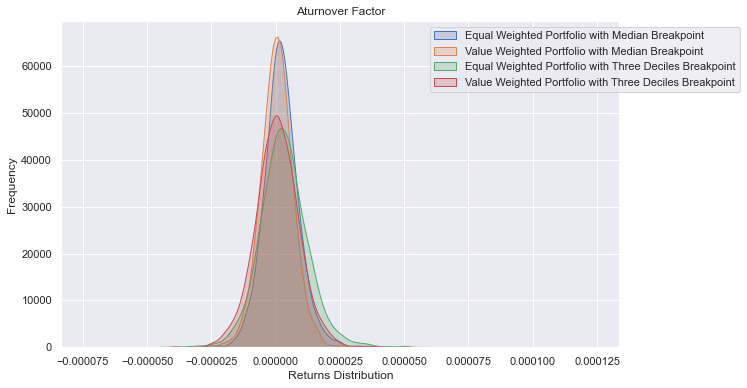
\includegraphics[scale=.63]{../../output/figures/aturnover.png}
	\label{fig:aturnover}
\end{figure}

\begin{figure}[H]
	\caption{Gmargins Factor Returns Distribution}
	\centering
	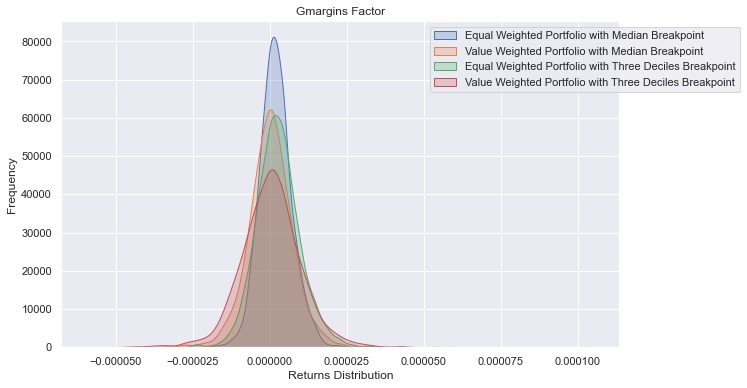
\includegraphics[scale=.63]{../../output/figures/gmargins.png}
	\label{fig:gmargins}
\end{figure}

\begin{figure}[H]
	\caption{Divp Factor Returns Distribution}
	\centering
	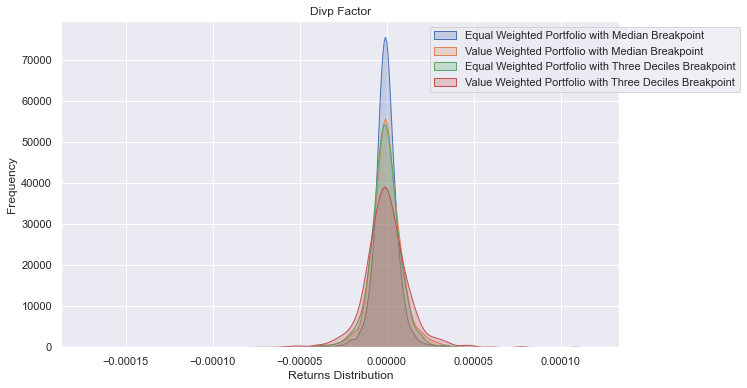
\includegraphics[scale=.63]{../../output/figures/divp.png}
	\label{fig:divp}
\end{figure}

\begin{figure}[H]
	\caption{Ep Factor Returns Distribution}
	\centering
	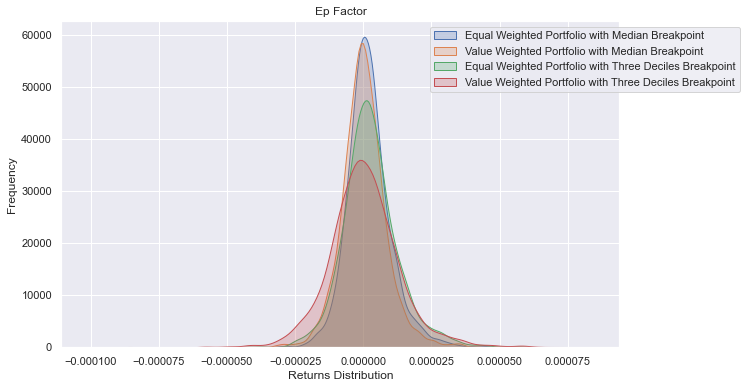
\includegraphics[scale=.63]{../../output/figures/ep.png}
	\label{fig:ep}
\end{figure}

\begin{figure}[H]
	\caption{Cfp Factor Returns Distribution}
	\centering
	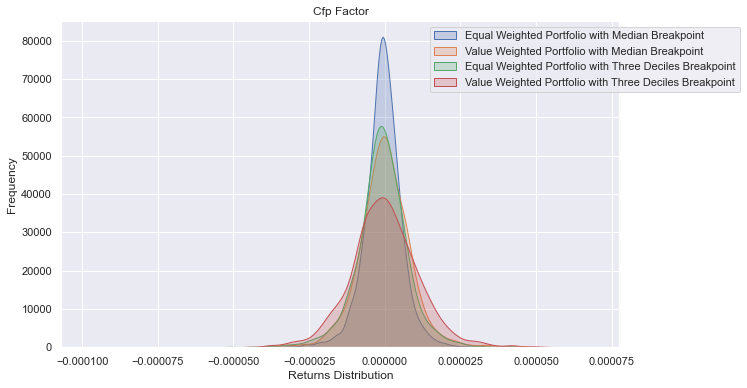
\includegraphics[scale=.63]{../../output/figures/cfp.png}
	\label{fig:cfp}
\end{figure}

\begin{figure}[H]
	\caption{Noa Factor Returns Distribution}
	\centering
	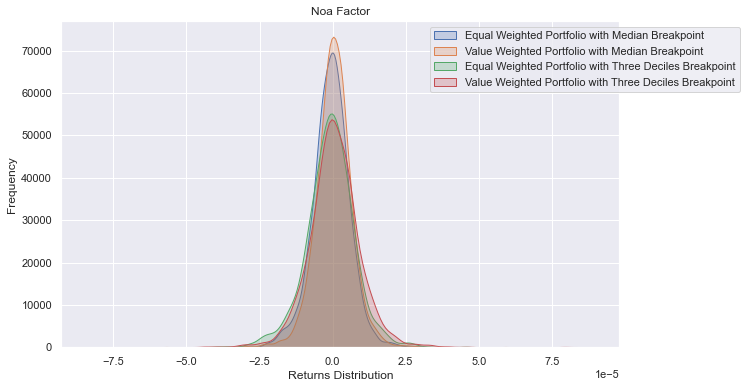
\includegraphics[scale=.63]{../../output/figures/noa.png}
	\label{fig:noa}
\end{figure}

\begin{figure}[H]
	\caption{Inv Factor Returns Distribution}
	\centering
	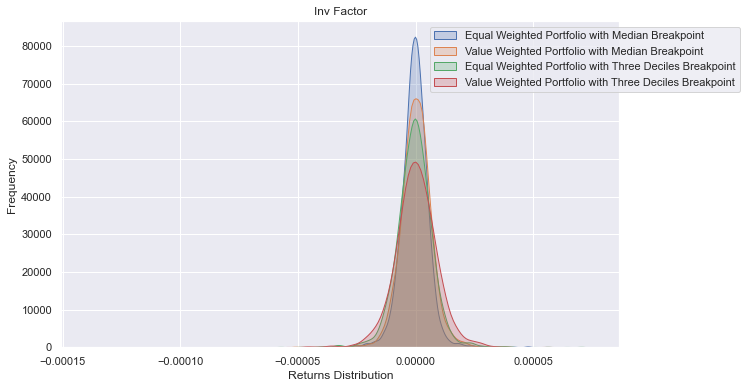
\includegraphics[scale=.63]{../../output/figures/inv.png}
	\label{fig:inv}
\end{figure}

\begin{figure}[H]
	\caption{Invcap Factor Returns Distribution}
	\centering
	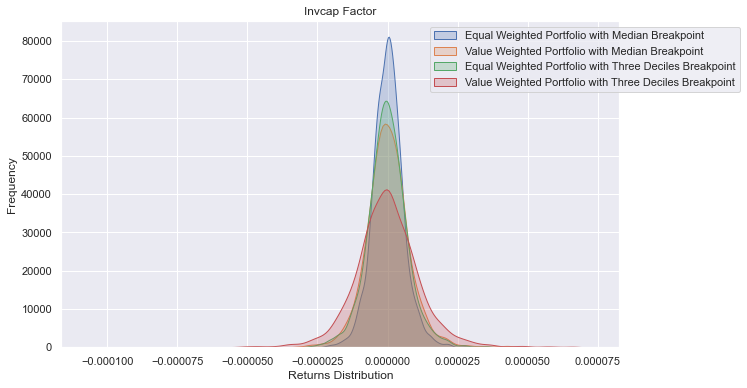
\includegraphics[scale=.63]{../../output/figures/invcap.png}
	\label{fig:invcap}
\end{figure}

\begin{figure}[H]
	\caption{Igrowth Factor Returns Distribution}
	\centering
	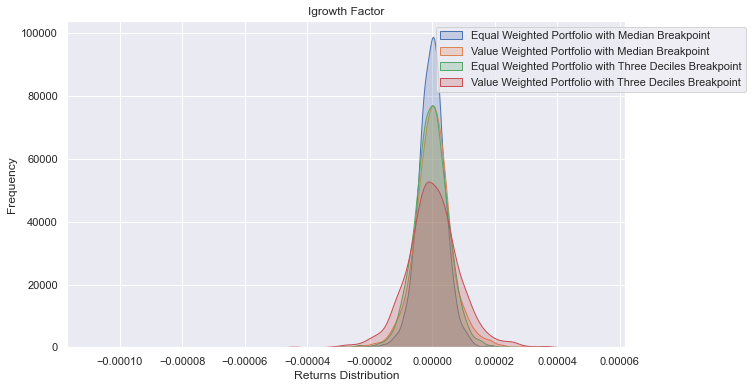
\includegraphics[scale=.63]{../../output/figures/igrowth.png}
	\label{fig:igrowth}
\end{figure}

\begin{figure}[H]
	\caption{Sgrowth Factor Returns Distribution}
	\centering
	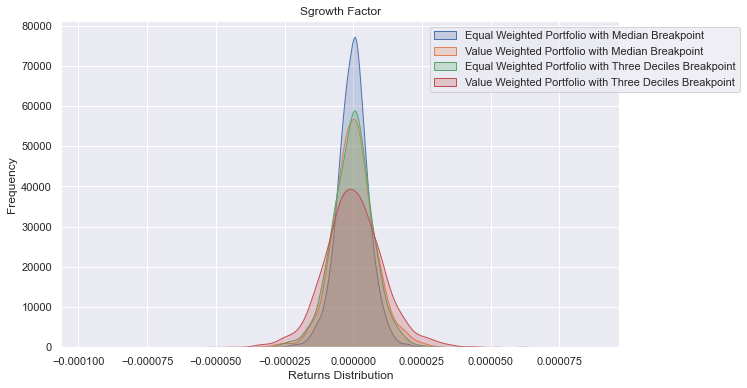
\includegraphics[scale=.63]{../../output/figures/sgrowth.png}
	\label{fig:sgrowth}
\end{figure}

\begin{figure}[H]
	\caption{Lev Factor Returns Distribution}
	\centering
	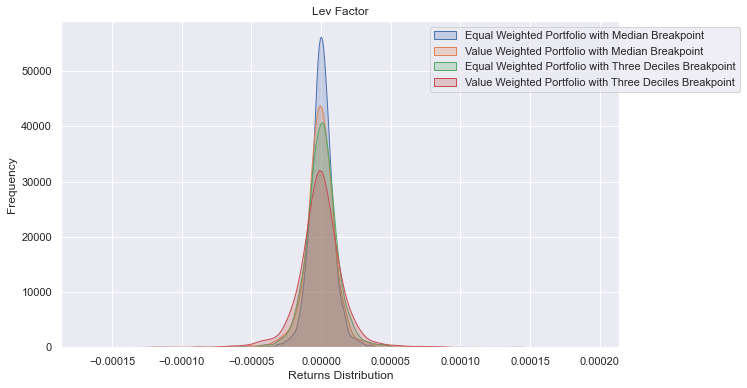
\includegraphics[scale=.63]{../../output/figures/lev.png}
	\label{fig:lev}
\end{figure}

\begin{figure}[H]
	\caption{Roaa Factor Returns Distribution}
	\centering
	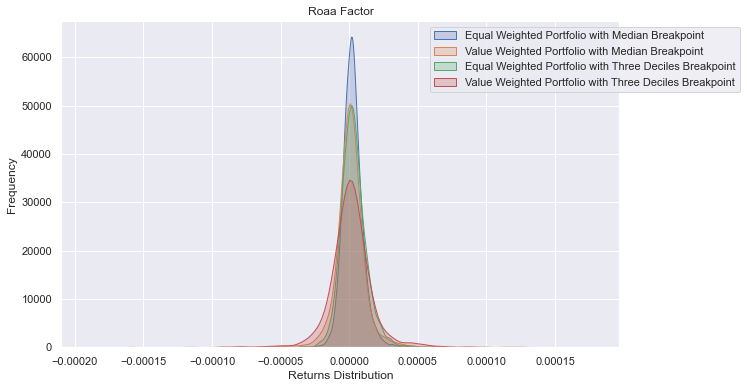
\includegraphics[scale=.63]{../../output/figures/roaa.png}
	\label{fig:roaa}
\end{figure}

\begin{figure}[H]
	\caption{Roea Factor Returns Distribution}
	\centering
	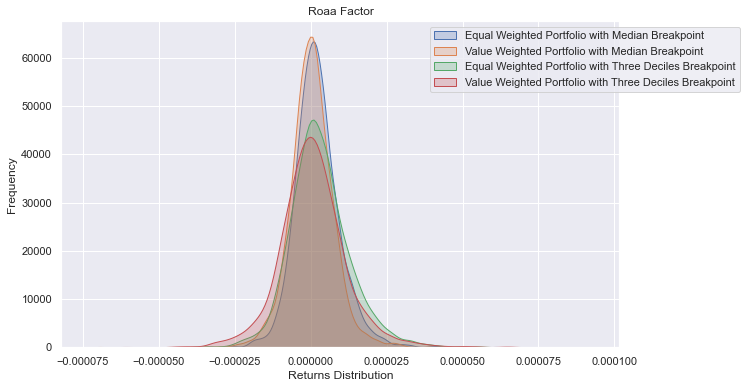
\includegraphics[scale=.63]{../../output/figures/roea.png}
	\label{fig:roea}
\end{figure}

\begin{figure}[H]
	\caption{Sp Factor Returns Distribution}
	\centering
	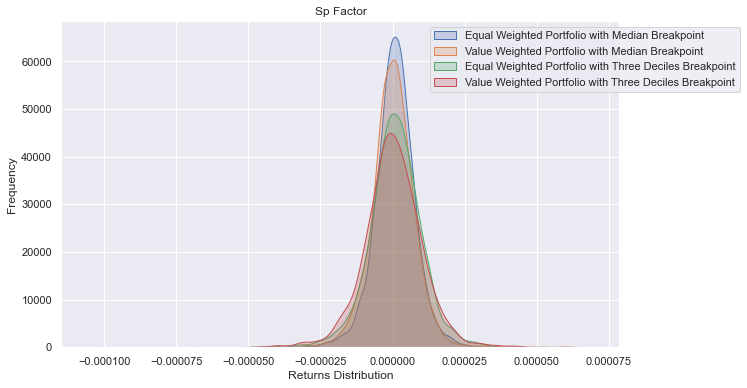
\includegraphics[scale=.63]{../../output/figures/sp.png}
	\label{fig:sp}
\end{figure}

\begin{figure}[H]
	\caption{Gltnoa Factor Returns Distribution}
	\centering
	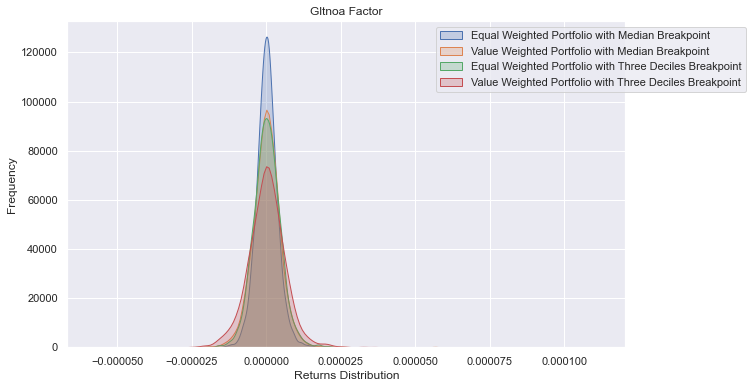
\includegraphics[scale=.63]{../../output/figures/gltnoa.png}
	\label{fig:gltnoa}
\end{figure}

\begin{figure}[H]
	\caption{Divg Factor Returns Distribution}
	\centering
	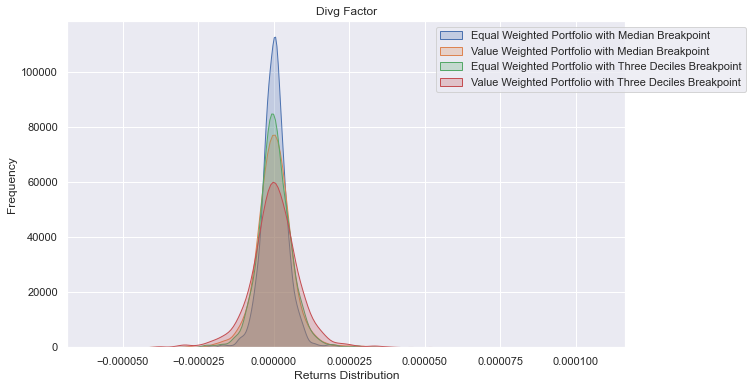
\includegraphics[scale=.63]{../../output/figures/divg.png}
	\label{fig:divg}
\end{figure}

\begin{figure}[H]
	\caption{Invaci Factor Returns Distribution}
	\centering
	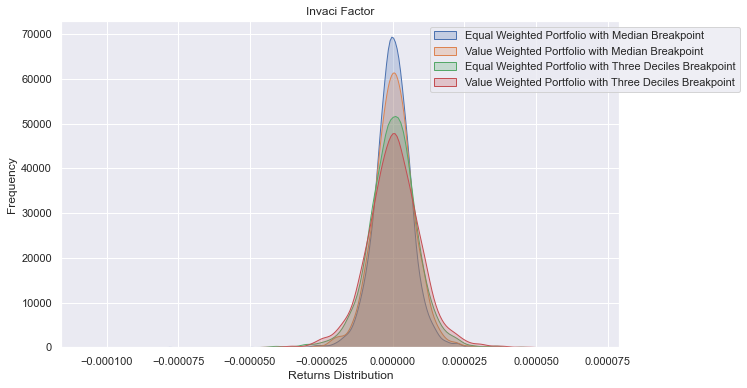
\includegraphics[scale=.63]{../../output/figures/invaci.png}
	\label{fig:invaci}
\end{figure}

\begin{figure}[H]
	\caption{Mom Factor Returns Distribution}
	\centering
	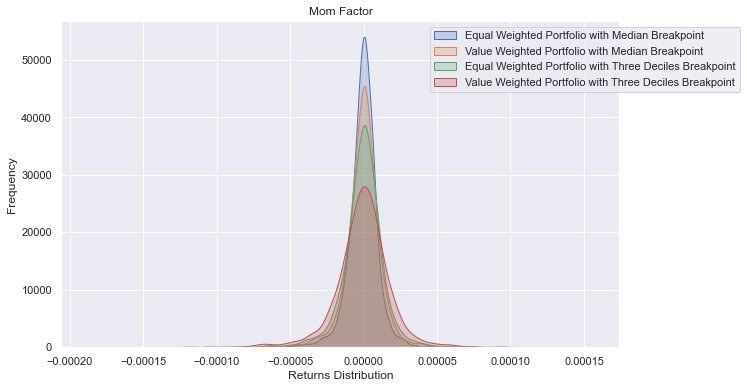
\includegraphics[scale=.63]{../../output/figures/mom.png}
	\label{fig:mom}
\end{figure}

\begin{figure}[H]
	\caption{Indmom Factor Returns Distribution}
	\centering
	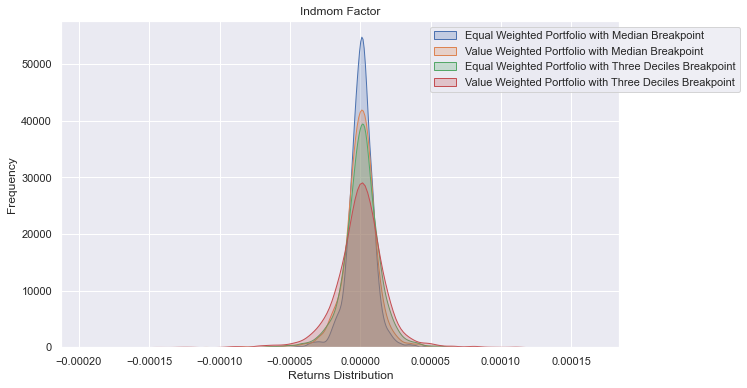
\includegraphics[scale=.63]{../../output/figures/indmom.png}
	\label{fig:indmom}
\end{figure}

\begin{figure}[H]
	\caption{Valmom Factor Returns Distribution}
	\centering
	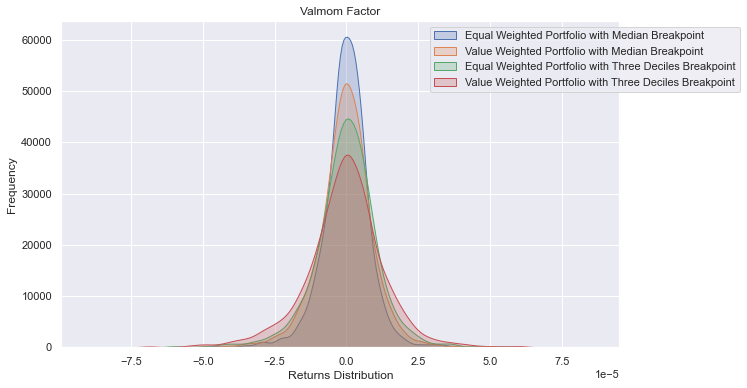
\includegraphics[scale=.63]{../../output/figures/valmom.png}
	\label{fig:valmom}
\end{figure}

\begin{figure}[H]
	\caption{Valmomprof Factor Returns Distribution}
	\centering
	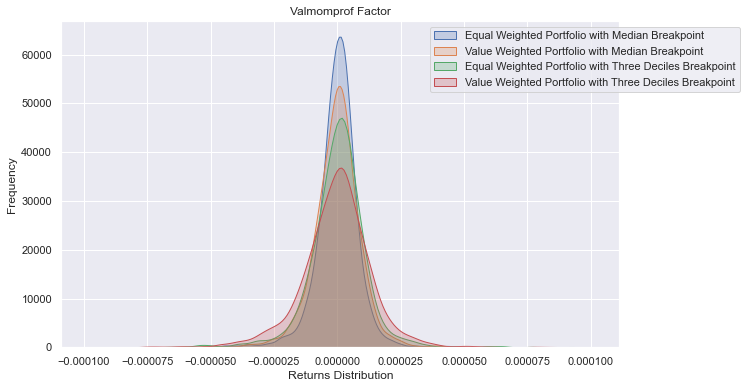
\includegraphics[scale=.63]{../../output/figures/valmomprof.png}
	\label{fig:valmomprof}
\end{figure}

\begin{figure}[H]
	\caption{Shortint Factor Returns Distribution}
	\centering
	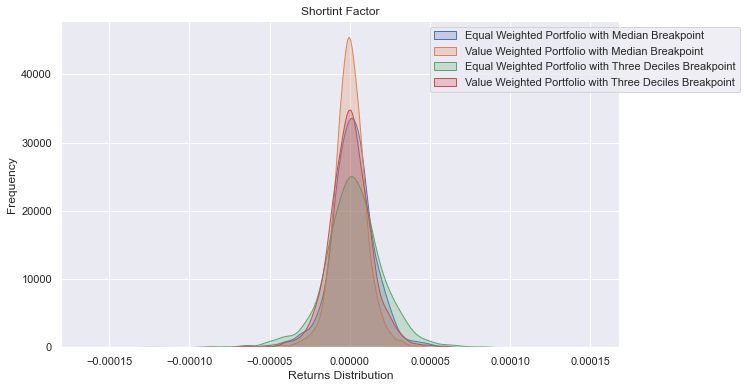
\includegraphics[scale=.63]{../../output/figures/shortint.png}
	\label{fig:shortint}
\end{figure}

\begin{figure}[H]
	\caption{Mom12 Factor Returns Distribution}
	\centering
	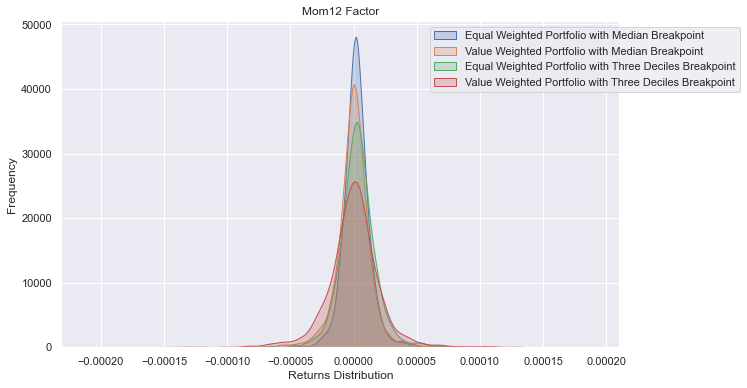
\includegraphics[scale=.63]{../../output/figures/mom12.png}
	\label{fig:mom12}
\end{figure}

\begin{figure}[H]
	\caption{Momrev Factor Returns Distribution}
	\centering
	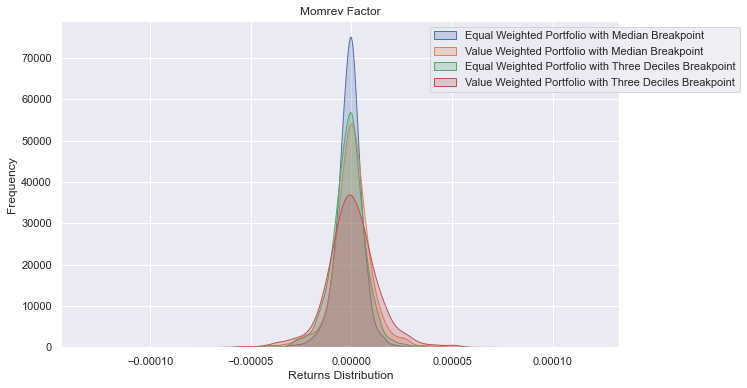
\includegraphics[scale=.63]{../../output/figures/momrev.png}
	\label{fig:momrev}
\end{figure}

\begin{figure}[H]
	\caption{Lrrev Factor Returns Distribution}
	\centering
	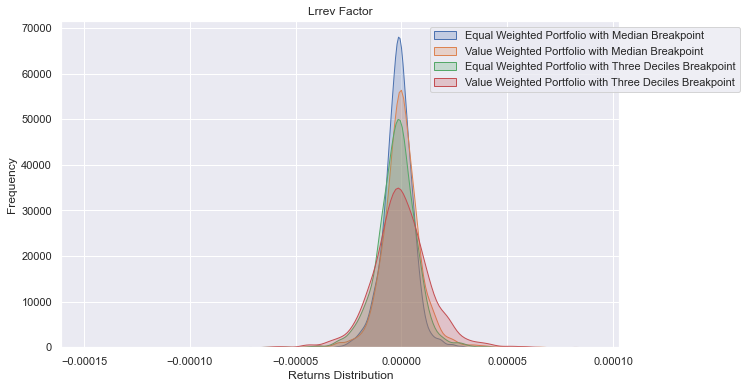
\includegraphics[scale=.63]{../../output/figures/lrrev.png}
	\label{fig:lrrev}
\end{figure}

\begin{figure}[H]
	\caption{Valuem Factor Returns Distribution}
	\centering
	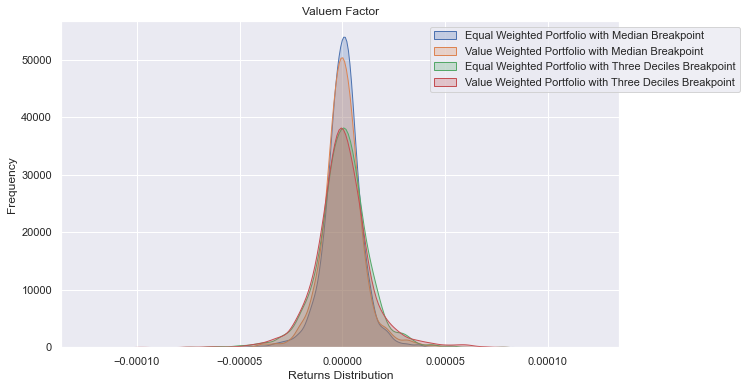
\includegraphics[scale=.63]{../../output/figures/valuem.png}
	\label{fig:valuem}
\end{figure}

\begin{figure}[H]
	\caption{Nissm Factor Returns Distribution}
	\centering
	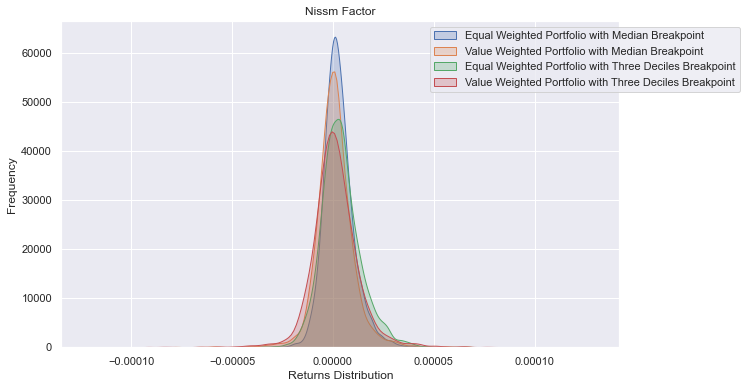
\includegraphics[scale=.63]{../../output/figures/nissm.png}
	\label{fig:nissm}
\end{figure}

\begin{figure}[H]
	\caption{Sue Factor Returns Distribution}
	\centering
	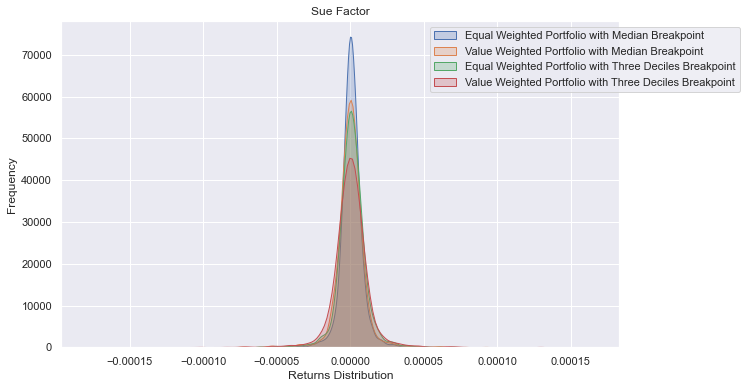
\includegraphics[scale=.63]{../../output/figures/sue.png}
	\label{fig:sue}
\end{figure}

\begin{figure}[H]
	\caption{Roe Factor Returns Distribution}
	\centering
	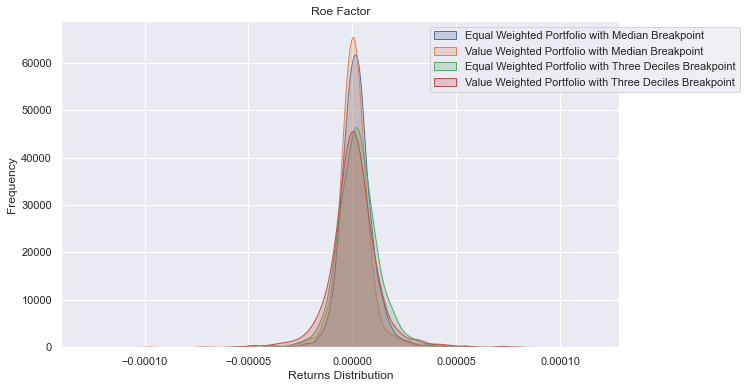
\includegraphics[scale=.63]{../../output/figures/roe.png}
	\label{fig:roe}
\end{figure}

\begin{figure}[H]
	\caption{Rome Factor Returns Distribution}
	\centering
	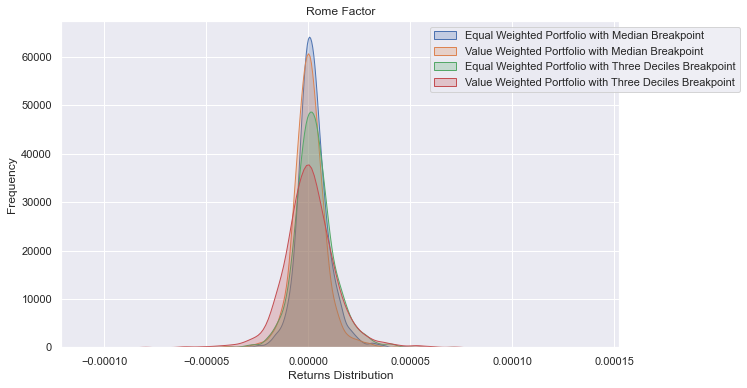
\includegraphics[scale=.63]{../../output/figures/rome.png}
	\label{fig:rome}
\end{figure}

\begin{figure}[H]
	\caption{Roa Factor Returns Distribution}
	\centering
	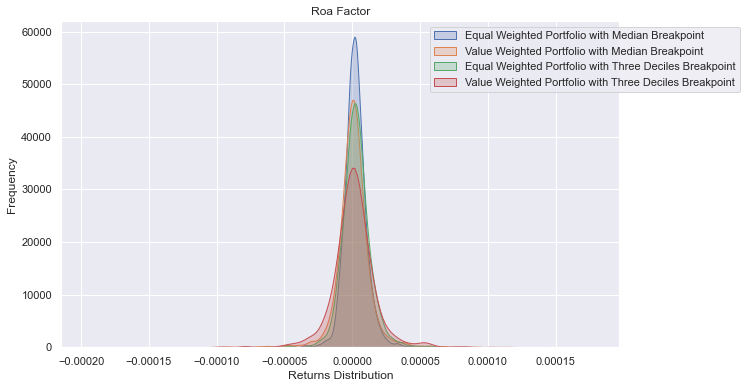
\includegraphics[scale=.63]{../../output/figures/roa.png}
	\label{fig:roa}
\end{figure}

\begin{figure}[H]
	\caption{Strev Factor Returns Distribution}
	\centering
	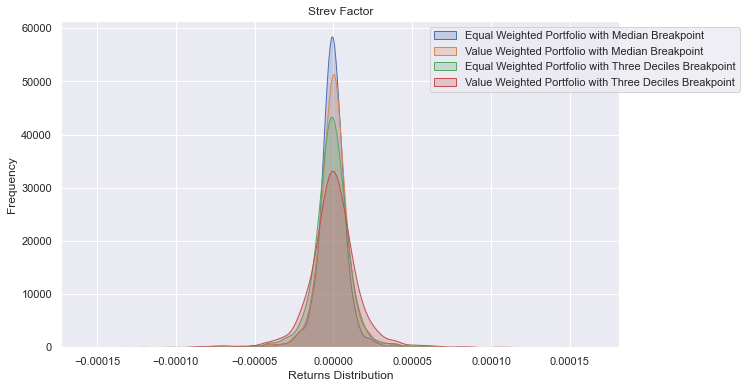
\includegraphics[scale=.63]{../../output/figures/strev.png}
	\label{fig:strev}
\end{figure}

\begin{figure}[H]
	\caption{Ivol Factor Returns Distribution}
	\centering
	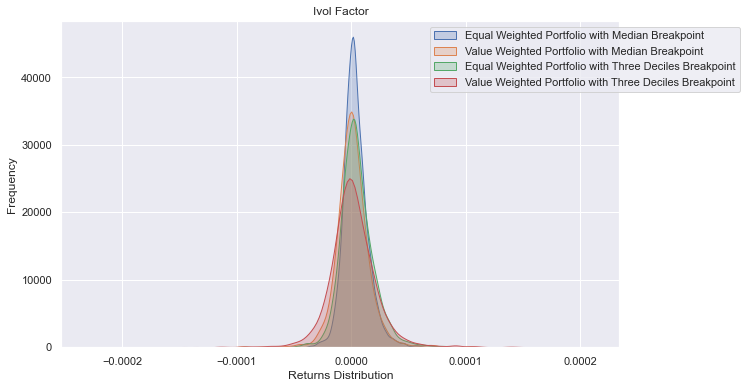
\includegraphics[scale=.63]{../../output/figures/ivol.png}
	\label{fig:ivol}
\end{figure}

\begin{figure}[H]
	\caption{Betaarb Factor Returns Distribution}
	\centering
	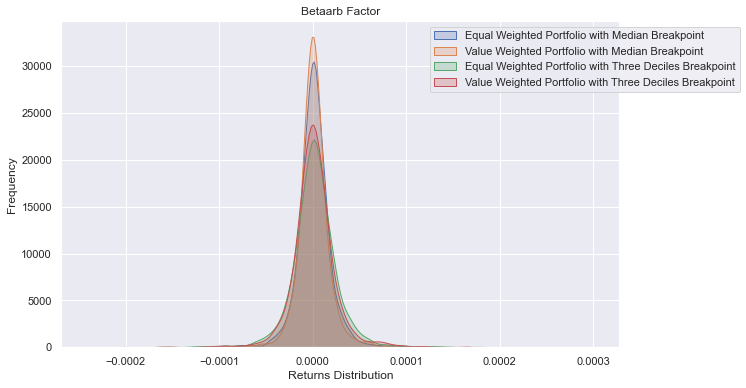
\includegraphics[scale=.63]{../../output/figures/betaarb.png}
	\label{fig:betaarb}
\end{figure}

\begin{figure}[H]
	\caption{Season Factor Returns Distribution}
	\centering
	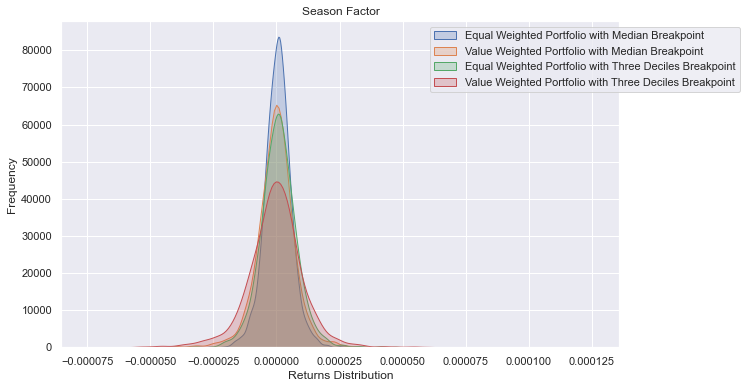
\includegraphics[scale=.63]{../../output/figures/season.png}
	\label{fig:season}
\end{figure}

\begin{figure}[H]
	\caption{Indrrev Factor Returns Distribution}
	\centering
	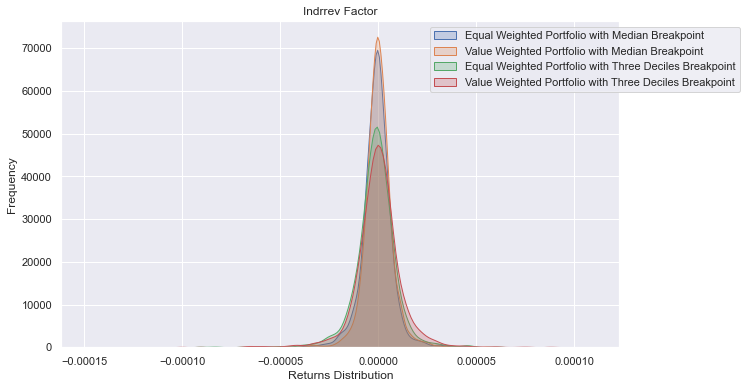
\includegraphics[scale=.63]{../../output/figures/indrrev.png}
	\label{fig:indrrev}
\end{figure}

\begin{figure}[H]
	\caption{Indrrevlv Factor Returns Distribution}
	\centering
	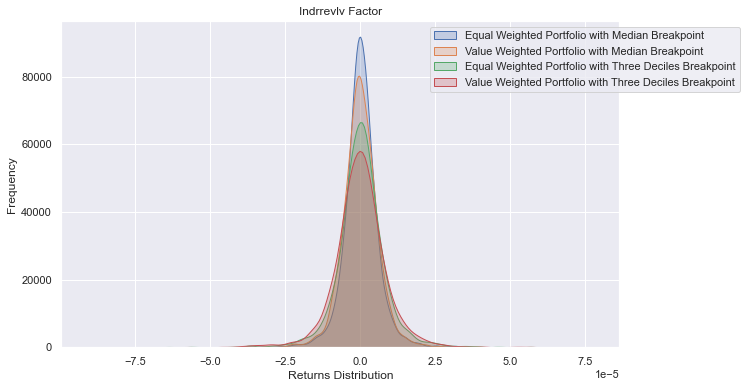
\includegraphics[scale=.63]{../../output/figures/indrrevlv.png}
	\label{fig:indrrevlv}
\end{figure}

\begin{figure}[H]
	\caption{Indmomrev Factor Returns Distribution}
	\centering
	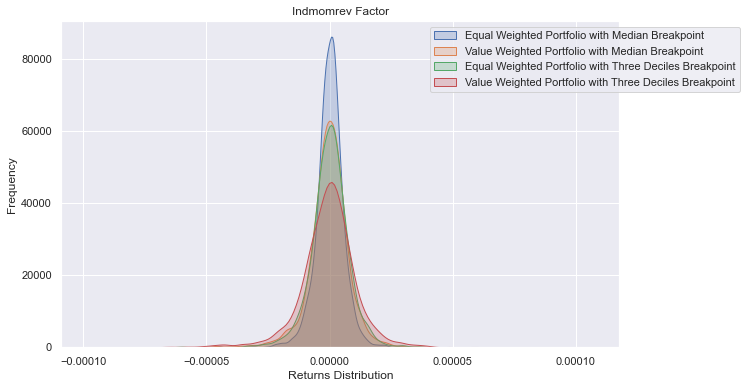
\includegraphics[scale=.63]{../../output/figures/indmomrev.png}
	\label{fig:indmomrev}
\end{figure}

\begin{figure}[H]
	\caption{Ciss Factor Returns Distribution}
	\centering
	\includegraphics[scale=.63]{../../output/figures/ciss.png}
	\label{fig:ciss}
\end{figure}

\begin{figure}[H]
	\caption{Price Factor Returns Distribution}
	\centering
	\includegraphics[scale=.63]{../../output/figures/price.png}
	\label{fig:price}
\end{figure}

\begin{figure}[H]
	\caption{Age Factor Returns Distribution}
	\centering
	\includegraphics[scale=.63]{../../output/figures/age.png}
	\label{fig:age}
\end{figure}

\begin{figure}[H]
	\caption{Shvol Factor Returns Distribution}
	\centering
	\includegraphics[scale=.63]{../../output/figures/shvol.png}
	\label{fig:shvol}
\end{figure}

\begin{figure}[H]
	\caption{Exchsw Factor Returns Distribution}
	\centering
	\includegraphics[scale=.63]{../../output/figures/exchsw.png}
	\label{fig:exchsw}
\end{figure}

\begin{figure}[H]
	\caption{Ipo Factor Returns Distribution}
	\centering
	\includegraphics[scale=.63]{../../output/figures/ipo.png}
	\label{fig:ipo}
\end{figure}





% TABLES
%\newpage
%\subsection{Tables}
%
%\begin{table}[H]
%\caption{}
%\centering
%\begin{threeparttable}
%%\input{../../output/}
%\end{threeparttable}
%\label{tab:}
%\end{table}






%% PORTUGUESE VERSION
%
%O LASSO é um procedimento categorizado dentro do conjunto de regressões penalizadas. O Penalized Least Squares é um procedimento de estimação que adiciona ao OLS um componente que penaliza os coeficientes fracos. O estimador de Penalized Least Squares é obtido através
%
%\begin{align*}
%	\widehat{\boldsymbol{\beta}}(\lambda)=\underset{\boldsymbol{\beta} \in \mathcal{B}}{\arg \min }\left[\sum_{i=1}^n\left(Y_i-\boldsymbol{\beta}^{\prime} \boldsymbol{X}_i\right)^2+\sum_{j=1}^p p_\lambda\left(\left|\beta_j\right| ; \boldsymbol{\alpha}, \text { data }\right)\right]
%\end{align*}
%
%onde $p_\lambda\left(\left|\beta_j\right| ; \boldsymbol{\alpha}, \text{data}\right)$ é uma função penalidade não negativa indexada pelo parâmetro de regularização $\lambda$ e poderia depender tanto dos dados quanto de hiper-parâmetros adicionais. Por exemplo,
%
%\begin{itemize}
%	\item Ridge
%	
%	$p_\lambda\left(\left|\beta_j\right| ; \boldsymbol{\alpha}\right.$, data $)=\lambda\left|\beta_j\right|^2$
%	\item LASSO
%	
%	$p_\lambda\left(\left|\beta_j\right| ; \boldsymbol{\alpha}\right.$, data $)=\lambda\left|\beta_j\right|$
%	\item LASSO e Ridge combinado
%	
%	$p_\lambda\left(\left|\beta_j\right| ; \boldsymbol{\alpha}\right.$, data $)=\alpha \lambda\left|\beta_j\right|+(1-\alpha) \lambda\left|\beta_j\right|^2$
%\end{itemize}
%
%O parâmetro de regularização $\lambda$ controla o número de parâmetros no modelo. Se $\lambda = \infty$, então nenhum parâmetro entra no modelo, e se $\lambda = 0$, então os parâmetros são simplesmente estimadores OLS.



\end{document}